%%%%%%%%%%%%%%%%%%%%%%%%%%%%%%%%%%%%%%%%%%%%%%%%%%%%%%%%%%%%%%%%%%%%%%%%%%%%%%%%
%                    Capitulo 8: Experimentacion                               %
%%%%%%%%%%%%%%%%%%%%%%%%%%%%%%%%%%%%%%%%%%%%%%%%%%%%%%%%%%%%%%%%%%%%%%%%%%%%%%%%

\chapter{Experimentación}

Una vez que el sistema ha sido implementado y validado, es necesario realizar un estudio
de su funcionamiento. Este estudio consiste en llevar a cabo una serie de experimentos,
los cuales pretenden poner a prueba dos aspectos fundamentales del sistema:

\begin{enumerate}
    \item La capacidad que tiene para generar problemas \texttt{PDDL} de forma
    automática a partir de los estados del juego.
    \item La capacidad que tiene para responder a los cambios dinámicos que
    se producen en los juegos.
\end{enumerate}

Para llevar a cabo estos experimentos se han escogido los siguientes juegos:

% Comentar aquí los juegos, relacionandolos con las imagenes
\begin{itemize}[label=\textbullet]
    \item \textbf{\textit{Boulderdash}}. El objetivo del juego consiste en recoger 9 de
    las gemas que hay esparcidas a lo largo de todo el mapa y llegar a la salida
    sin morir en el intento (ver figura \ref{fig:boulderdash}). En el mapa hay también
    esparcidos dos tipos de enemigos: las mariposas y los cangrejos, los cuales matarán al agente
    si chocan con él. Si dos enemigos chocan entre sí, se generará una gema nueva. En el
    juego original, las rocas son afectadas por la gravedad, de manera que si la casilla debajo de una
    de ellas está excavada (es decir, es una casilla vacía), la roca caerá hasta toparse
    con una casilla que contenga tierra, un muro, una gema u otra roca. Una roca cayendo puede matar
    al agente si colisiona con este. Sin embargo, debido a la extrema dificultad que supone
    simular este sistema de físicas en un dominio \texttt{PDDL}, se trabaja con una versión
    simplificada del juego donde las rocas no caen y pueden ser excavadas utilizando el pico
    del que dispone el agente, de forma que estas rocas desaparecen del mapa.
    
    Esta versión del juego, a pesar de ser simplificada, es no determinista, ya que el
    comportamiento de los enemigos es totalmente aleatorio. Este no determinismo introduce
    por tanto cierto dinamismo en el juego, ya que los enemigos pueden interponerse en el
    camino del agente y matarlo. Es aquí donde el monitor va a jugar un papel clave,
    ya que gracias a él se podrá determinar si algún enemigo se interpone entre el agente
    y el objetivo al que se dirige.
    
    \item \textbf{\textit{Ice and Fire}}. En este juego, el agente tiene que atravesar una especie
    de laberinto hasta la salida, el cual está lleno de obstáculos como pinchos, fuego y hielo
    (ver figura \ref{fig:ice_and_fire}). Estos obstáculos matarán al jugador si entra en contacto
    directo con ellos. Sin embargo, las casillas que contienen fuego pueden ser atravesadas si el
    agente dispone de unas botas de fuego. Análogamente, se pueden atravesar las casillas que
    contienen hielo si se tienen las botas de hielo. Se pueden llevar equipados los dos tipos
    de botas simultáneamente, de forma que se pueden atravesar ambos tipos de obstáculos. Los
    pinchos, por desgracia, no pueden atravesarse. A lo largo del mapa hay también una serie
    de monedas que pueden ser recogidas para aumentar la puntuación del jugador, aunque esto es más
    bien secundario. Este juego es totalmente determinista ya que, al no haber enemigos u otros
    personajes en el mapa, no se pueden llegar a producir eventos exógenos que obliguen a modificar
    un plan obtenido.
    
    \item \textbf{\textit{Labyrinth Dual}}. Aquí el agente también tiene que atravesar un laberinto
    hasta la salida esquivando los pinchos y atravesando una serie de casillas para las que requiere
    un traje en específico de los que se pueden encontrar por el mapa (ver figura \ref{fig:labyrinth_dual}).
    El traje rojo permite atravesar los muros de color gris oscuro y el traje azul permite atravesar
    las muros de color azul. El agente solo puede llevar equipado un traje a la vez. Si ya tiene equipado
    uno y coge el otro, se cambia de traje, perdiendo la capacidad de atravesar las casillas que
    antes podía. Por tanto, hay que tener cierto cuidado a la hora de coger un traje, ya que
    en algunas ocasiones cambiar de traje puede llegar a encerrar al agente, impidiéndole llegar
    a la meta. A pesar de eso, el juego es totalmente determinista, ya que no hay factores
    externos que puedan impedir que un plan hasta un objetivo determinado sea llevado a cabo.
\end{itemize}

\begin{figure}[H]
    \centering
    \begin{subfigure}[t]{.5\textwidth}
        \centering
        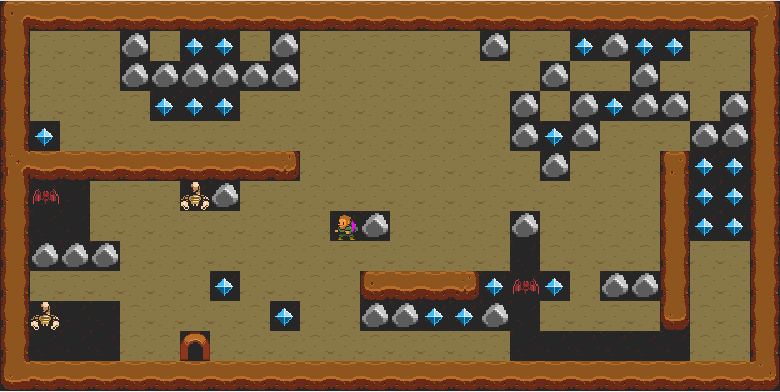
\includegraphics[scale=0.3]{img/CH08/boulderdash.png}
        \caption{\textit{Boulderdash}.}
        \label{fig:boulderdash}
    \end{subfigure}%
    \begin{subfigure}[t]{.5\textwidth}
        \centering
        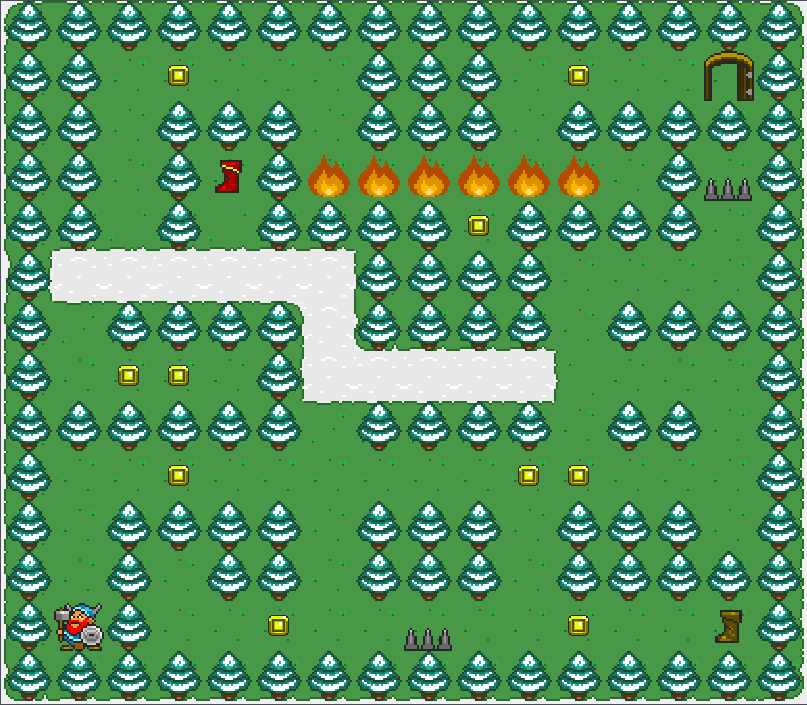
\includegraphics[scale=0.25]{img/CH08/ice_and_fire.png}
        \caption{\textit{Ice and Fire}.}
        \label{fig:ice_and_fire}
    \end{subfigure}
    \par\bigskip
    \begin{subfigure}[t]{0.5\textwidth}
        \centering
        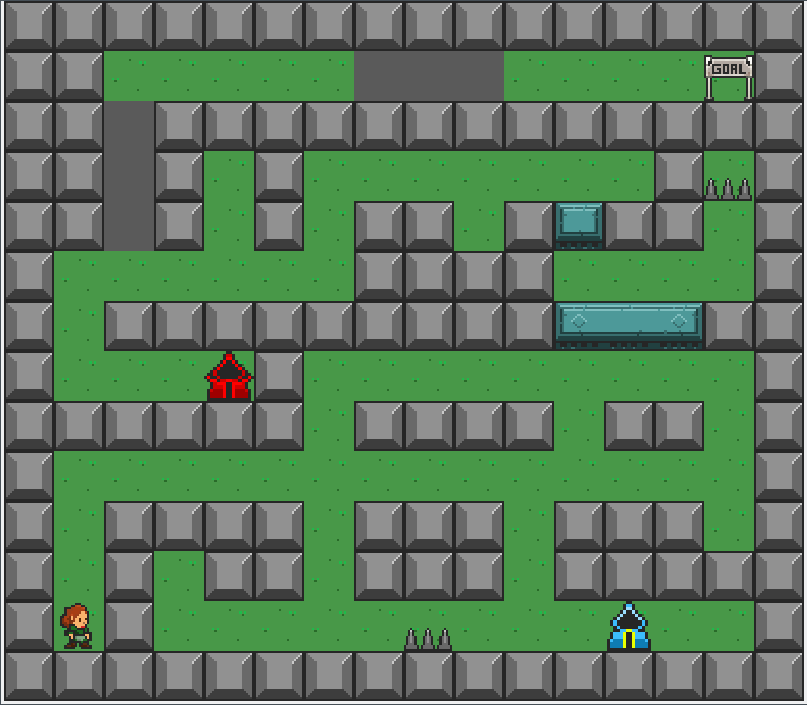
\includegraphics[scale=0.25]{img/CH08/labyrinth_dual.png}
        \caption{\textit{Labyrinth Dual}.}
        \label{fig:labyrinth_dual}
    \end{subfigure}
    \caption{Juegos con los que se han realizado los experimentos.}
    \label{fig:games}
\end{figure}

Para cada juego se ha creado su dominio \texttt{PDDL}, intentando hacer una representación lo más
fiel posible del juego. En la tabla \ref{tab:info-domains} puede el número de predicados, de tipos y
de acciones que conforman cada uno de los dominios. Adicionalmente, debido a que la planificación es
un proceso lento, es importante destacar que a la hora de construir el sistema se han modificado tanto el
tiempo máximo que tiene el agente para dar una respuesta, el cual ha pasado a ser 40 segundos (originalmente 40
milisegundos), como el tiempo máximo que se espera antes de descalificar al agente, el cual es ahora
500 segundos (anteriormente 50 milisegundos).

\begin{table}[H]
\centering
\begin{tabular}{|c|ccc|}
\hline
\textbf{Juego} & \textbf{Predicados} & \textbf{Tipos} & \textbf{Acciones} \\ \hline
\textit{Boulderdash} & 15 & 9 & 17 \\ \hline
\textit{Ice and Fire} & 13 & 10 & 14 \\ \hline
\textit{Labyrinth Dual} & 12 & 9 & 14 \\ \hline
\end{tabular}
\caption{Información sobre los dominios creados para cada juego.}
\label{tab:info-domains}
\end{table}

\section{Generación de problemas}

Para comprobar la generación de problemas se han hecho pruebas con cada uno de los cinco
niveles de los tres juegos anteriormente mencionados. Para cada nivel de cada juego se ha
creado un archivo de configuración en el cual se ha especificado la información correspondiente,
además de decir los objetivos concretos que se deben alcanzar en cada nivel. En cada ejecución se
ha obtenido información del número de predicados y objetos que que conforman el estado inicial
del primer archivo de problema generado\footnote{En general, va a haber muy poca variabilidad entre
dichos números para archivos de problema posteriores, y como en algunos juegos hay más
elementos al principio del juego, esto nos da una idea de cuánto se tarda en generar el problema más
grande.}, el tiempo total de ejecución desde que empieza el juego, el tiempo de generación
de los predicados de conectividad entre casillas, el tiempo medio de traducción de
un estado de observación, el tiempo medio de generación un archivo de problema
y la suma de los tres tiempos anteriores, lo cual nos da una idea de cuánto se tarda en
generar un problema completo de media. Se han realizado 3 ejecuciones de cada nivel, de modo
que los resultados obtenidos para los tiempos son una media de esas tres ejecuciones.

En la tabla \ref{tab:exp-results} se pueden ver los resultados obtenidos. Como puede observarse,
en todos los casos se generan problemas con más de 1000 predicados y cerca de 350-400 objetos.
Puede verse también que el tiempo medio total para generar un problema es del orden de centésimas
de segundo. Generar problemas de este tamaño a mano podría llevar días e incluso semanas, además de
que se pueden cometer errores a la hora de crearlos, lo cual puede retrasar dicha creación aún
más tiempo. Por tanto, hacer uso de esta arquitectura permite ahorrar muchísimo tiempo de trabajo
y permite detectar de forma más rápida los posibles errores que puedan aparecer a la hora de crear
un archivo de problema.

Si observamos los tiempos individuales que suman dicho tiempo total de generación de problema, se
puede ver que las fases de traducción del estado de observación y la generación del archivo
de problema tienen un tiempo medio del orden de milésimas de segundo, mientras que el proceso
que más tarda es la generación de los predicados de conectividad, el cual tarda un tiempo medio
del orden de las centésimas de segundo. Esto es normal, ya que los predicados de conectividad representan
una gran parte de los predicados del problema. Para un mapa dado de tamaño $w \times h$, siendo $w$
la anchura y $h$ la altura, el número de predicados de conectividad, $PC$, viene dado por la expresión
\eqref{eq:pc}:

\begin{equation}
    PC = 4 \cdot 2 \; pred + 2 ((w-2) + (h-2)) \cdot 3 \; pred + (w-2)(h-2) \cdot 4 \; pred
    \label{eq:pc}
\end{equation}

\begin{landscape}
\begin{table}[]
\centering
\resizebox{1.51\textwidth}{!}{%
\begin{tabular}{|c|c|cccccccc|}
\hline
\textbf{Juego} &
  \textbf{Nivel} &
  \textbf{Objetivos} &
  \textbf{\begin{tabular}[c]{@{}c@{}}Predicados problema\\ inicial\end{tabular}} &
  \textbf{\begin{tabular}[c]{@{}c@{}}Objetos problema\\ inicial\end{tabular}} &
  \textbf{\begin{tabular}[c]{@{}c@{}}Tiempo medio\\ ejecución (s)\end{tabular}} &
  \textbf{\begin{tabular}[c]{@{}c@{}}Tiempo medio\\ generación predicados\\ conectividad (s)\end{tabular}} &
  \textbf{\begin{tabular}[c]{@{}c@{}}Tiempo medio\\ traducción estado\\ de observación (s)\end{tabular}} &
  \textbf{\begin{tabular}[c]{@{}c@{}}Tiempo medio\\ generación archivo\\ de problema (s)\end{tabular}} &
  \textbf{\begin{tabular}[c]{@{}c@{}}Tiempo medio total\\ generación problema\\ (s)\end{tabular}} \\ \hline
\multirow{5}{*}{\textit{Boulderdash}}    & \textbf{0} & 10 & 1735 & 400 & 0.4967 & 0.0313 & 0.0024 & 0.0038 & 0.0375 \\ \cline{2-10} 
                                         & \textbf{1} & 10 & 1721 & 393 & 0.428  & 0.0323 & 0.0029 & 0.0039 & 0.0392 \\ \cline{2-10} 
                                         & \textbf{2} & 10 & 1717 & 391 & 0.5293 & 0.0347 & 0.0034 & 0.0044 & 0.0425 \\ \cline{2-10} 
                                         & \textbf{3} & 10 & 1733 & 399 & 0.7487 & 0.0327 & 0.0049 & 0.0048 & 0.0423 \\ \cline{2-10} 
                                         & \textbf{4} & 10 & 1731 & 398 & 0.4403 & 0.0317 & 0.0030 & 0.0039 & 0.0386 \\ \hline
\multirow{5}{*}{\textit{Ice and Fire}}   & \textbf{0} & 3  & 1215 & 391 & 0.417  & 0.027  & 0.0026 & 0.003  & 0.0326 \\ \cline{2-10} 
                                         & \textbf{1} & 3  & 1234 & 410 & 0.4827 & 0.0307 & 0.0028 & 0.0056 & 0.0390 \\ \cline{2-10} 
                                         & \textbf{2} & 3  & 1235 & 411 & 0.522  & 0.0273 & 0.0031 & 0.0045 & 0.0349 \\ \cline{2-10} 
                                         & \textbf{3} & 3  & 1219 & 395 & 0.4587 & 0.0323 & 0.0029 & 0.0061 & 0.0413 \\ \cline{2-10} 
                                         & \textbf{4} & 3  & 1210 & 386 & 0.697  & 0.0273 & 0.0031 & 0.0055 & 0.0359 \\ \hline
\multirow{5}{*}{\textit{Labyrinth Dual}} & \textbf{0} & 3  & 1085 & 369 & 0.4503 & 0.0303 & 0.0029 & 0.0043 & 0.0376 \\ \cline{2-10} 
                                         & \textbf{1} & 2  & 1069 & 380 & 0.3847 & 0.0303 & 0.0027 & 0.0045 & 0.0376 \\ \cline{2-10} 
                                         & \textbf{2} & 3  & 1073 & 378 & 0.4107 & 0.0287 & 0.0024 & 0.0029 & 0,0339 \\ \cline{2-10} 
                                         & \textbf{3} & 3  & 1083 & 376 & 0.41   & 0.0297 & 0.0031 & 0.0052 & 0.038  \\ \cline{2-10} 
                                         & \textbf{4} & 2  & 1079 & 363 & 0.5623 & 0.029  & 0.0029 & 0.0062 & 0.0381 \\ \hline
\end{tabular}%
}
\caption{Resultados de la experimentación.}
\label{tab:exp-results}
\end{table}
\end{landscape}

\section{Respuesta a cambios dinámicos}

Para facilitar el estudio de la respuesta que ofrece el sistema a los cambios dinámicos en
los juegos, se ha creado un nuevo nivel del juego \textit{Boulderdash}, que es el
único de la lista que contiene no determinismo al tener enemigos que se mueven por el mapa
aleatoriamente, y se ha fijado una semilla aleatoria, de forma que el comportamiento de los enemigos
fuese el deseado. El nuevo nivel puede observarse en la figura \ref{fig:discrepancy_1}. Se ha creado
también un archivo de configuración en el cual se han especificado qué gemas tiene que coger
el agente antes de salir del nivel. La primera de ellas es la gema que está justo encima suyo,
la cual está rodeada de enemigos.

Después de obtener un plan hasta dicha gema, comienza la ejecución de éste. Mientas el agente
intenta avanzar, una mariposa se le cruza en el camino, tal y como puede verse en la figura
\ref{fig:discrepancy_2}. El monitor, al hacer un estudio de las precondiciones de la siguiente
acción a ejecutar, detecta una discrepancia, ya que la celda justo arriba del agente está
ocupada por un enemigo, algo que no se esperaba. Es entonces cuando se le indica al gestor
de objetivos que se ha producido una discrepancia y que se debe seleccionar un nuevo objetivo,
que resulta ser la gema que se encontraba a la izquierda de la posición inicial del agente.

Se obtiene un plan hasta dicha gema y, tal y como se puede ver en la figura \ref{fig:discrepancy_3},
el agente alcanza el nuevo objetivo propuesto. Vemos por tanto que el agente ha conseguido
responder a la aparición de un enemigo en su camino, algo que no estaba previsto cuando obtuvo
el plan, deteniendo por tanto la ejecución del plan actual y cambiando a un nuevo objetivo.

\begin{figure}[H]
    \centering
    \begin{subfigure}[t]{0.32\textwidth}
        \centering
        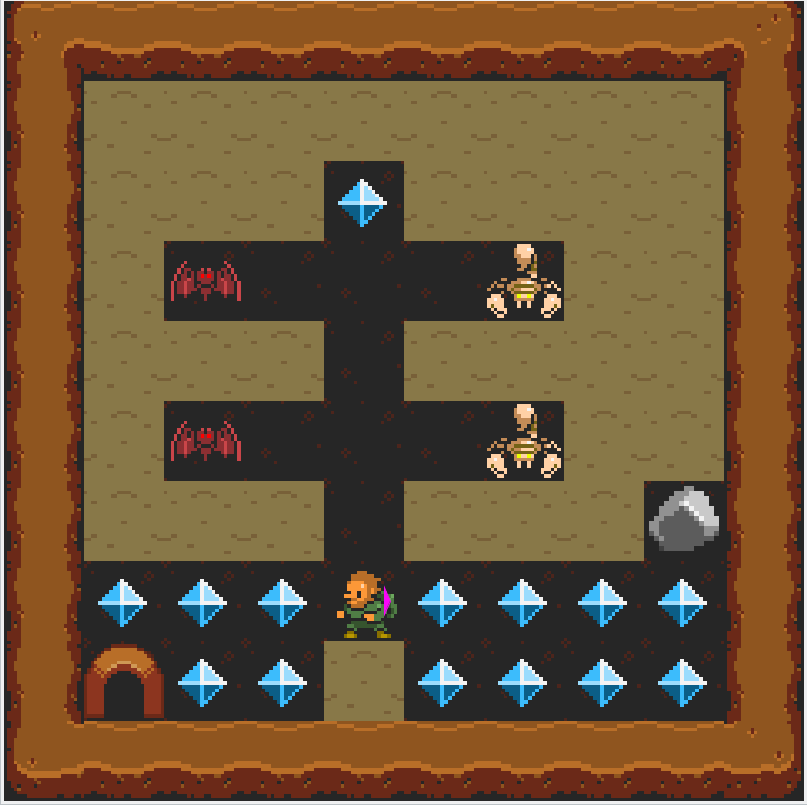
\includegraphics[scale=0.2]{img/CH08/discrepancy_1.png}
        \caption{Estado inicial del juego.}
        \label{fig:discrepancy_1}
    \end{subfigure}%
    \begin{subfigure}[t]{0.32\textwidth}
        \centering
        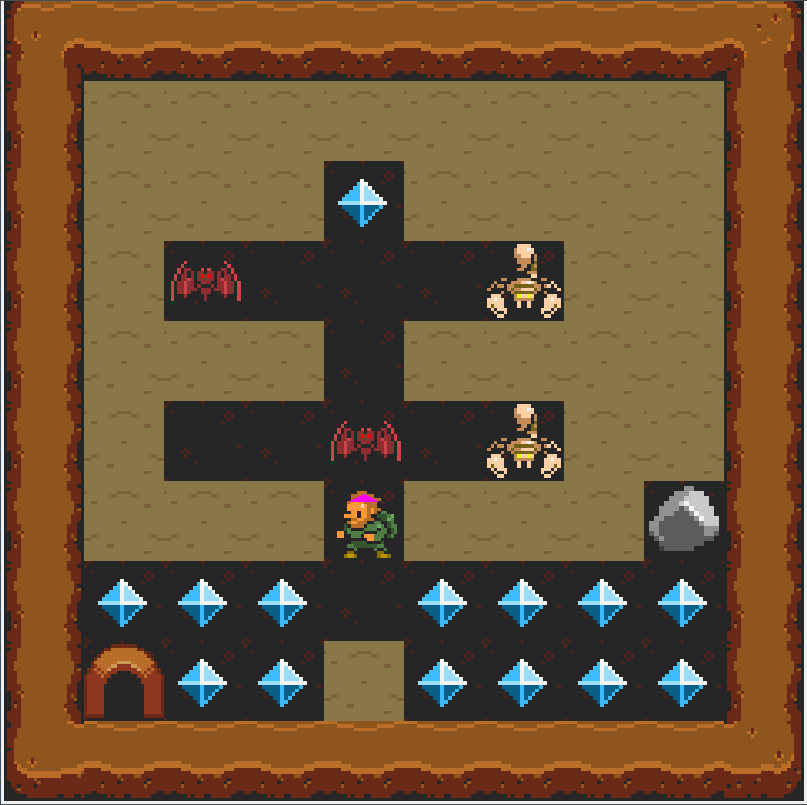
\includegraphics[scale=0.2]{img/CH08/discrepancy_2.png}
        \caption{Mariposa bloquea el camino.}
        \label{fig:discrepancy_2}
    \end{subfigure}%
    \begin{subfigure}[t]{0.32\textwidth}
        \centering
        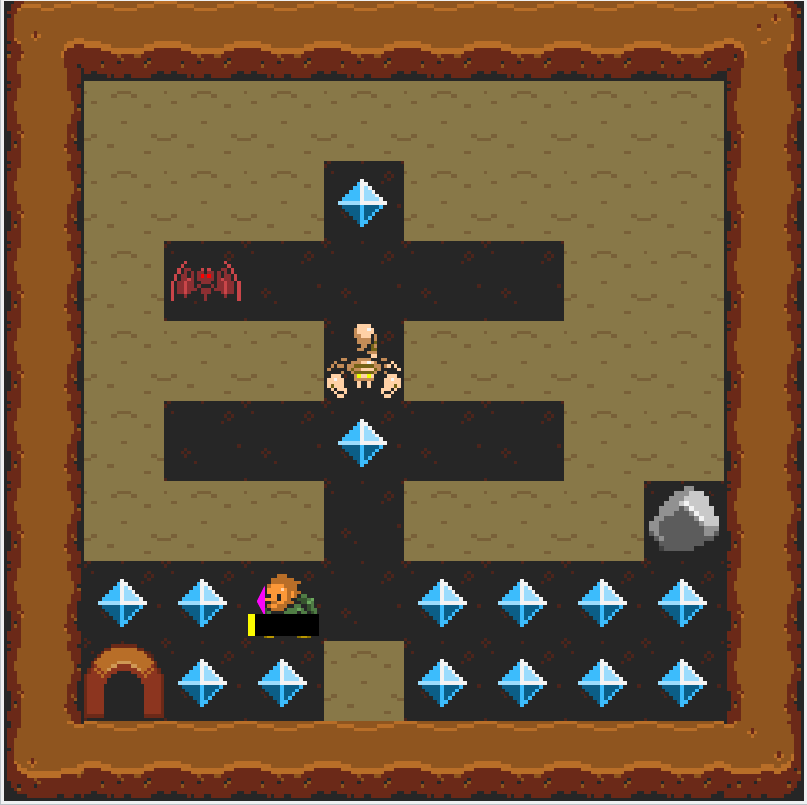
\includegraphics[scale=0.2]{img/CH08/discrepancy_3.png}
        \caption{Agente cambia de objetivo y lo alcanza.}
        \label{fig:discrepancy_3}
    \end{subfigure}
    \caption{Ejemplo de respuesta a cambios dinámicos en el entorno en \textit{Boulderdash}.}
    \label{fig:discrepancies}
\end{figure}